\documentclass{article}
\usepackage{hyperref}

%Russian-specific packages
%--------------------------------------
\usepackage[T2A]{fontenc}
\usepackage[utf8]{inputenc}
\usepackage[russian]{babel}

%--------------------------------------

%Hyphenation rules
%--------------------------------------
\usepackage{hyphenat}
\hyphenation{ма-те-ма-ти-ка вос-ста-нав-ли-вать}
%--------------------------------------

\title{Приватность в блокчейне}
\author{Михаил Койпиш }
\date{Декабрь 2018}

\usepackage{natbib}
\usepackage{graphicx}
\usepackage{algorithmicx}
\usepackage{algpseudocode}
\usepackage{algorithm}

\begin{document}

\maketitle

\section{Введение}
There is a theory which states that if ever anyone discovers exactly what the Universe is for and why it is here, it will instantly disappear and be replaced by something even more bizarre and inexplicable.
There is another theory which states that this has already happened.

\begin{figure}[h!]
\centering
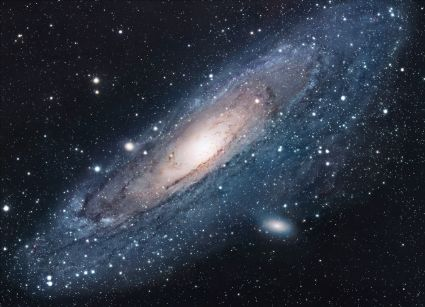
\includegraphics[scale=1.7]{universe}
\caption{The Universe}
\label{fig:universe}
\end{figure}

\section{Конфиденциальные транзакции в Bitcoin}

{\bf Описание Bitcoin}.
Bitcoin является децентрализованной БД, осуществляющей платежную систему.
Пользователь Bitcoin идентифицируется открытым ключом, являющимся его \textit{адресом}, или псевдонимом в системе,
и обладает секретным личным ключом, позволяющим авторизовать его действия в системе~--- подписывать транзакции.
Сеть Bitoin в каждый момент времени хранит информацию о том, сколько и кому принадлежит денег,
в определенной форме~--- \textit{UTXO (Unspent Transactions Outputs)}.
Отдельный UTXO (выход транзакции, выходная запись) представляет собой пару $(address, amount)$,
означающую что $amount$ денег принадлежит $address$.
Глобальная таблица UTXO (состояние сети Bitcoin) представляет собой список отдельных UTXO.
Отметим, что в этой таблице не запрещается повторение адресов (то есть возможно несколько UTXO с тем же адресом).
\footnote{Кажется странным, почему бы такие UTXO не аггрегировать по адресу.
Тогда таблица была бы компактнее,
а пользоваться ей было бы проще (адреса в таблице уникальные). Но такой дизайн выбран не просто так.
Дело в том, что на самом деле UTXO хранится не таблицей, а деревом Меркле,
что позволяет ``тонким'' клиентам
получать компактные доказательства содержания определенного UTXO в БД.
Так как новые UTXO появляются постепенно (в результате выполнения транзакций),
то в дерево Меркле проще добавить новую запись, чем редактировать существующую.
В то же время, необходима операция удаления UTXO из БД.}

Транзакция Bitcoin по сути представляет собой сообщение от пользователя,
называемого \textit{автором транзакции}
\footnote{Опустим здесь сложный случай мульти-подписей и множественные авторов транзакции.},
о том, чтобы вывести из глобальной таблицы принадлежащие ему определенные UTXO,
называемые \textit{входами транзакции},
и поместить в глобальную таблицу новые UTXO (с определенными адресами и суммами),
называемые \textit{выходами транзакции}.
Адреса выходов определяют \textit{получателей}. Автор может назначить получателями
как себя так и произвольные адреса, принадлежащие другим пользователям (и
даже не принадлежащие никому).
\footnote{Для простоты, опустим здесь обязательные второстепенные выходы любой транзакции~---
вознаграждение майнера и эмиссия денег.}
Естественно, транзакция должна быть подписана автором,
все входы должны принадлежать автору, входы должны содержаться в глобальной таблице,
 и суммы входов и выходов должны совпадать.
Если эти условия выполнены, БД принимает транзакцию, и изменяет глобальную таблицу UTXO.
Несложно видеть, что этих правил достаточно для осуществления корректной работы
системы электронных денег и переводов. В частности, условие неотрицательных сумм и
условие сохранения баланса вместе обеспечивают невозможность потратить больше,
чем есть (у пользователя в его UTXO).
Условие того, что выполнение транзакции приводит к удалению входного UTXO
из глобальной таблицы, обеспечивает защиту от двойной траты (double spending).


\floatname{algorithm}{Description}
\begin{algorithm}
\begin{algorithmic}
\caption{Bitcoin State}
\item Список UTXO:
\item $U_1, U_2, \ldots$,
\item каждый из которых представляет собой пару адрес-сумма.
\item Далее в будем использовать обозначения $U_i.address$ и $U_i.amount$

\end{algorithmic}
\end{algorithm}

\begin{algorithm}
\begin{algorithmic}
\caption{Bitcoin Transaction Structure}
\item $I_1, I_2, \ldots I_n$ - входные UTXO,
\item $O_1, O_2, \ldots O_n$ - выходные UTXO,
\item $a$ - автор (его адрес),
\item $\sigma_a$ - подпись автора транзакции.
\end{algorithmic}
\end{algorithm}

\begin{algorithm}
\caption{Bitcoin Transaction Verification}
\begin{itemize}
  \item
  State.contains($I_i.address$) $\forall i$~--- все входы содержатся в глобальной таблице UTXO;
  \item
  $I_i.address = a, \forall i$~--- входные UTXO принадлежат автору транзакции;
  \item
   $\sigma_a$~--- корректная подпись автора $a$;
  \item
  $\sum_{\forall i} {I_i.amount} = \sum_{\forall j} {O_j.amount}$~--- денежный баланс сохранен;
  \item
  $ \forall j, O_j.amount \ge 0$~--- отсутсвуют отрицательные балансы на выходе.
\end{itemize}
\end{algorithm}

\begin{algorithm}
\caption{Bitcoin Transaction Effect}
\begin{itemize}
  \item
  State.remove($I_i$) $\forall i$~--- все входные UTXO удаляются из глобальной таблицы;
  \item
  State.add($O_j$) $\forall j$~--- все выходные UTXO добавляются в глобальную таблицу;
\end{itemize}
\end{algorithm}

{\bf Приватность}.
 Благодаря тому, что сообщение-транзакция в открытом виде
содержит все детали денежного перевода (адрес отправителя и получателя, сумма),
а также тому, что состояние БД в открытом виде содержит все кошельники пользователей,
верифицировать и проводить транзакции может децентрализованный консенсус.
Однако, это полностью лишает пользователей приватности.

Существуют разные аспекты приватности. Обычно, скрытие участия пользователя
(в данном случае~--- в денежном переводе, в качестве отправителя, либо получателя)
 называют \textit{анонимностью}. Скрытие же содержания (в данном случае~--- сумма перевода;
 либо общая сумма, принадлежащая пользователю)  обычно называют \textit{конфиденциальностью}.
Так, в Bitcoin нарушена как анонимность
\footnote{ В Bitcoin обеспечевается некоторая степень анонимности, так называется \textit{псевдонимность},
благодаря тому, что идентифактор пользователя (адрес) произвольно выбирается самим пользователем,
причем нет необходимости его где-либо регистрировать. Однако, несложно показать, что такая анонимность
довольно хрупкая.}
 так и конфиденциальность.

 На первый взгляд кажется, что отсутствие приватности является прямым следствием
 открытой верифицируемости, и совместить децентрализованность системы с приватностью невозможно.
 Действительно, если мы будем как-то скрывать (зашифровывать, не указывать) адреса в транзакциях, как определить что
 данный пользователь имеет доступ к данному UTXO?
 Аналогично, как проверить баланс сумм входов и выходов, если сумма в транзакции скрыта?


 Оставив пока что анонимность, попробуем решить проблему конфиденциальности~---
 сделать суммы транзакций скрытыми от всех, кроме автора (очевидно) и получателя.
 Если получателей несколько~-- каждый из них должен видеть только сумму предназначенного ему UTXO.
 В то же время, транзакция должна оставаться публично верифицируемой,
 и эффект проведения транзакции должен изменить состояние корректно~--- отправитель больше не обладает
 этими UTXO, в то время как получатели (и только они) смогут распоряжаться полученными UTXO в будущем.
 При этом, желательно достичь \textit{опциональной конфиденциальности}.
 То есть, при необходимости, автор (или получатель) может раскрыть детали транзакции для
 третьих лиц, причем без необходимости раскрывать свои личные ключи.
 Такая возможность окажется полезной в суде/арбитраже.

  Представим, что конфиденциальный UTXO (далее~--- cUTXO) по-прежнему включает
  в себя адрес в открытом виде,
 но вместо суммы $a$ хранит ее некоторый ``образ'' $C_k(a)$,
 созданный с помощью некоторого ключа $k$, выбираемого автором транзакции, в которой был создан сUTXO.
 По образу невозможно (в каком-либо смысле, например в вычислительном) найти сумму,
 однако обладатель ключа может проверить, что данный образ соответсвует данной сумме.
 Образы устроены таким образом, что позволяют публично проверять баланс сумм,
 а также выявлять отрицательные суммы.
 Однако создать доказательство можно лишь обладая ключами от образов,
 иначе можно было бы достаточно легко раскрыть сумму любого образа.
 Таким образом, автор, обладающий не только личным ключом, но и ключами от образов входов,
  создает верифицируемую транзакцию, в том числе выбирая ключи образов выходов.
 Чтобы получатель перевода смог потратить предназначенные ему cUTXO,
 автор транзакции сообщает ему ключи от образов
 \footnote{Он может это сделать с помощью любых каналов связи, обеспечиващих конфиденциальность.
 Самый простой вариант~--- просто зашифровать на открытом ключе (адресе) получателя и приложить к транзакции.
 Для этого, конечно необходимо, чтобы ключи пользователей могли использоваться как для подписи так и для шифрования.
 В Bitcoin это так.}.

Действительно, такую схему можно реализовать. Схема CT (Confidential Transactions)
будет описана чуть позже, а пока, чтобы двигаться дальше,
будут описаны некоторые криптографические примитивы, необходимые для построения CT.

{\bf Коммитмент Педерсена}.
Схемой коммитмента называется криптографический примитив, позволяющий зафиксировать
некоторое секретное значение, не разглашая его.
Позже, когда обладатель секретного значения пожелает раскрыть его,
он может предъявить доказательство соответствия раскрытого значения и коммитмента.
Дадим здесь полуформальное определение.
\textit{Коммитментом} секретного значения $x$ с рандомизируещим фактором $r$
называется строка $C = Comm(x, r)$ для некоторой функции $Comm$.
Функция $Comm$ такова,
 что выполняются следующие требования:
\begin{itemize}
  \item
   \textit{сокрытие (hiding)}~--- по коммитменту $C = Comm(x,r)$ невозможно найти $x$;
   если невозможность заключается в вычислительной сложности, то говорят о
   \textit{вычислительном сокрытии (computational hiding)};
   если это принципиально невозможно (в силу того, что $Comm$ сюрьективна
   относительно $x$), то говорят о \textit{совершенном сокрытии (perfect hiding)};
  \item
  \textit{cвязывание (binding)}~--- по значениям $x$ и $r$,
  невозможно найти две пары значений $(x, r)$ и $(x', r')$ , такие что $x \neq x'$,
  и $Comm(x,r) = Comm(x', r')$;другими словами, невозможно найти коллизию в $Comm$;
  как и в случае сокрытия, различают вычислительный и совершенный варианты.
\end{itemize}

Например, любая криптографическая (односторонная, коллизионно-стойкая) хэш-функция $h$ является подходит
для схемы коммитмента: $Comm(x, r) = h(x \parallel r)$. В данном случае,
обеспечивается совершенное сокрытие и вычислительное связывание.

Интересной для нас является схема коммитмента Педерсена.
Пусть в группе $G$, в которой дискретное логарифмирование вычислительно сложно,
 выбраны два независимых
\footnote{Независимость означает что никому не известен дискретный логарифм одного генератора к другому.
Для этого достаточно выбирать каждый из генераторов случайно.
Как и другие долговременные параметры криптосистемы,
$h$ и $g$ следует генерировать на так называемой церемонии генерации долговременных параметров.
Проведение церемонии должно быть таким, чтобы честность не вызывала сомнений.}
 генератора $h$ и $g$. Для натуральных чисел $x$ и $r$,
 функция коммитмента определяется следующим образом:
 $$
 Comm(x, r) = h^x g^r.
 $$

 Несложно видеть, что коммитмент Педерсена обеспечивает совершенное сокрытие и вычислительное связывание.
 Что более интересно, коммитмент Педерсена обладает свойством \textit{гомоморфности}:

 $$
 Comm(x_1, r_1) \cdot Comm(x_2, r_2) = Comm(x_1 + x_2, r_1 + r_2).
 $$

Все три свойства коммитмента Педерсена (сокрытие, связывание и гомоморфность)
будут необходимы нам для реализации CT.

{\bf Кольцевые подписи}.

Кольцевые подписи это особый тип подписи,
позволяющий подписанту выработать подпись анонимно,
``скрываясь'' среди произвольной группы подписантов (произвольного списка открытых ключей).
При этом, в отличие от групповых подписей,
отсутсвуют так называемые менеджеры группы,
т.е. группа может быть выбрана подписантом произвольно,
без чьего-либо согласия. Проверяющий подпись сможет удостовериться,
что подпись выработана на одном из ключей определенной группы,
однако непонятно на каком именно (равновероятно на любом из группы).

Приведем пример одной из самых простых схем кольцевой подписи,
предложенной вместе с самой концепцией кольцевых подписей в знаменитой статье \cite{ringSig}.

Пусть имеется семейство односторонних c потайным входом перестановок (one-way trapdoor permutation)
$F: \{0,1\}^l \mapsto \{0,1\}^l$, а $d$~--- потайной вход (личный ключ),
позволяющий инвертировать $F$.
Например, подойдет RSA, с небольшими доработками
\footnote{Есть некоторая проблема в том,
что область определения и домен RSA с открытым ключом $(e, N)$ не совпадают с $\{0,1\}^l$,
и более того, будут отличаться от RSA с другим ключом $(e', N')$
(даже если $N$ и $N'$ имеют одинаковую длину в битовом представлении).
Для устранения этого неравенства используется некоторая надстройка над RSA.}.

Каждый потенциальный подписант $i$ обладает личным ключом $d_i$ и открытым ключом $P_i$,
определяющим перестановку $F_i$

Пусть также имется симметричный шифр $E_k: \{0,1\}^l \mapsto \{0,1\}^l$.

Подпись состоит из следующих списка открытых ключей $(P_1, P_2, \ldots, P_{n})$,
списка значений $(x_1, x_2, \ldots, x_{n}), x_i\in \{0,1\}^l$,
значения $v\in \{0,1\}^l$ и $k$.

Верификация подписи состоит в проверке следующего равенства:
$$
C_{k, v} (F_1(x_1), F_2(x_2), \ldots, F_n(x_n)) = v,
$$
где $С_{k, v}$ определяется следующим образом:
$$
C_{k,v}(y_1, \ldots, y_n) = E_k(y_n \oplus E_k(y_{n-1} \oplus (\ldots \oplus E_k(y_1 \oplus v)))).
$$

Алгоритм создания кольцевой подписи состоит в следующем.
Подписант выбирает группу анонимности~--- $n$ потенциальных подписантов,
включая себя.
Также, случайно выбирается ключ симметричного шифрования $k$.
Пусть $(P_1, P_2, \ldots, P_{n})$ - фиксированный список открытых ключей
потенциальных подписантов, среди который $P_s$~--- ключ настоящего подписанта.
Подписант также выбирает случайное значение $v\in \{0, 1\}^l$.
Несложно видеть, что обладая личным ключом $d_s$,
можно решить требуемое уравнение следующим образом:
\begin{enumerate}
  \item
  Выбрать случайно все $x_i$ кроме $i=s$, подставить соответсвующие $y_i = F_i(x_i)$
  в уравнение.
  \item
  Решить уравнение относительно $y_s$.
  \item
  Используя личный ключ $d_i$, инвертировать $F_s$ и найти $x_s$.
\end{enumerate}
\bibliographystyle{plain}
\bibliography{references}
\end{document}
